\subsection{Definitions}
\subsubsection*{Cutting Planes}\label{sec:def_cuttingplane}
A cutting plane is a plane which cuts the surface of a data set in two parts and hides one of these parts. (see \autoref{fig:cuttingplane_cube})

\begin{figure}[h!]
  \centering
  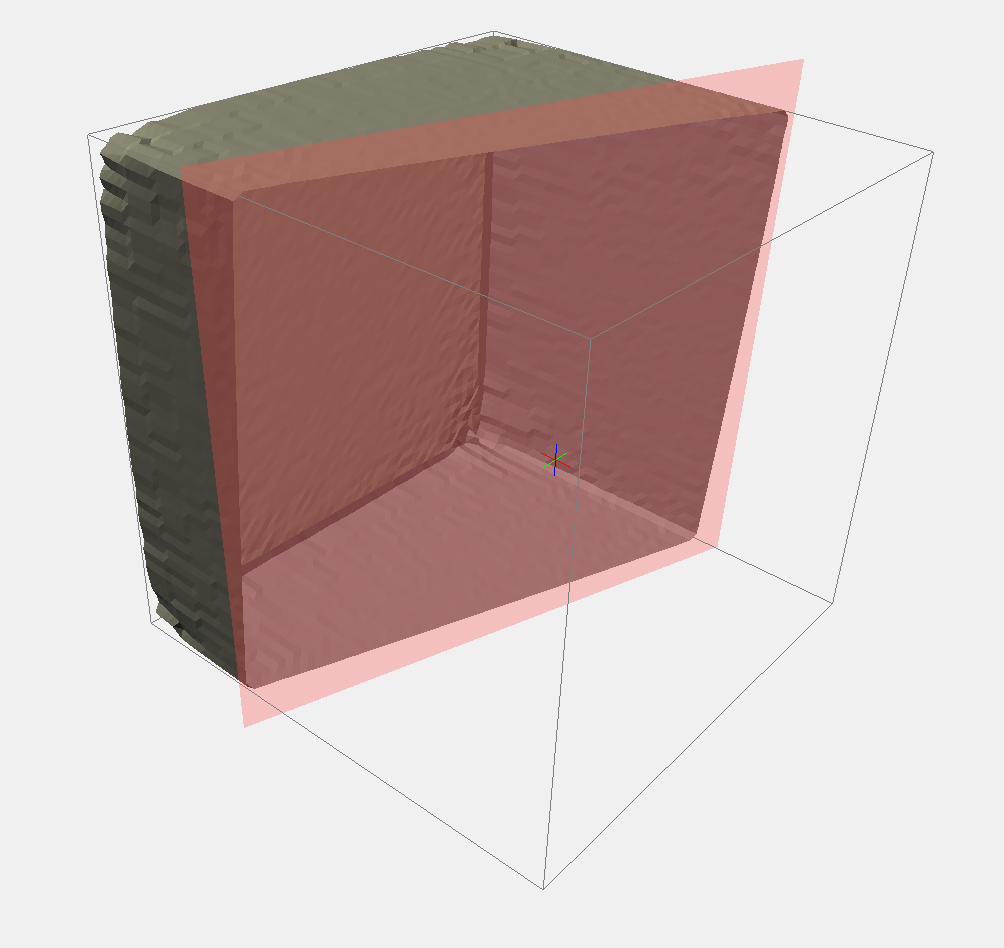
\includegraphics[width=1.0\textwidth]{img/cuttingplane_cube.png}
  \caption{A cutting plane cutting away the front part of a cube}
  \label{fig:cuttingplane_cube}
\end{figure}
